\section{判题沙箱的设计}
\subsection{总体分析}
判题沙箱是保证OJ系统安全的重要措施之一,如果没有沙箱,直接在服务器上运行用户的代码是存在严重安全风险\cite{wooyun-oj-vul}的,而且也无法去控制或获取代码的运行时间、占用内存大小和运行结果等运行数据。

沙箱要实现的功能:

\begin{itemize}
\item[-]获取进程运行实际时间和CPU时间,超时则结束进程
\item[-]获取代码运行占用的内存,超内存则结束进程
\item[-]获取代码运行结果和返回值
\item[-]阻止代码执行一切危险的动作
\end{itemize}

\subsubsection{进程实际运行时间和CPU时间}

一般情况下,一个进程实际运行时间与占用的CPU时间并不相等。在单核处理器上,任何时刻只有一个进程在真正的运行,其余的进程都在等待。操作系统会按照一定的算法进行调度,每个进程轮换的执行。这就导致进程实际运行时间必然大于CPU时间。所以说,一个进程运行的耗时还是需要统计CPU时间,实际运行时间受到系统负载的影响比较大。

\subsubsection{进程内存占用}

Linux下一个进程实际的内存占用的计算是比较复杂的,因为一个进程在运行的时候,其占用的内存并不是仅仅代码中变量占用的内存和动态分配的内存相加,还包括动态库占用、声明占用但未分配等等很多影响因素。

Linux上的\texttt{ps aux}命令,可以查看进程的内存占用,

\begin{verbatim}
virusdefender@vm:~$ ps aux
USER        PID %CPU %MEM    VSZ   RSS TTY      STAT START   TIME COMMAND
root          1  3.2  0.1  33900  4440 ?        Ss   11:20   0:02 /sbin/init
\end{verbatim}

需要注意的是RSS和VSZ两列。简单来说RSS就是进程实际占用的物理内存,VSZ是进程的虚拟内存,也就是进程还没有使用但是未来可能会分配的内存大小。如果把所有进程的RSS加起来,可能会超过实际的物理内存,那是因为动态库的共享内存在每个进程中都是重复计算的,而实际只需要占用一份内存空间。

\subsubsection{进程的状态和返回值}
进程结束的时候一般都有返回值的,比如

\begin{verbatim}
#include <stdlib.h>
#include <string.h>
int main()
{
    int *p = (int *)malloc(100000);
    if(p == NULL){
        exit(1);
    }
    memset(p, 0, 100000);
    return 0;
}
\end{verbatim}就会在分配内存成功的时候返回0,分配失败的时候返回1。

Linux上有一种signal的机制来进程进程间通信,进程可以自定义信号处理函数或者忽略信号,比如

\begin{verbatim}
#include <stdlib.h>
#include <string.h>
int main()
{
    memset(NULL, 0, 100000);
    return 0;
}
\end{verbatim}就会提示段错误,并且因为程序中没有捕获\texttt{SEGFAULT}的signal,导致进程被终止。我们可以通过这种机制来获取和控制进程状态。

\subsubsection{OJ上要避免的危险操作}

为了确保OJ运行环境的安全,沙箱需要控制用户代码可以执行的动作,常见的危险行为有:
\begin{itemize}
\item[-]使用汇编直接调用系统调用
\item[-]调用系统原生API,比如\texttt{remove("/etc/passwd")}
\item[-]执行系统命令,比如\texttt{system("rm –rf /")}
\item[-]恶意占用大量系统资源,比如\texttt{while(1){fork()}}
\item[-]网络通信相关,可能泄露服务器上敏感信息
\item[-]造成编译器出现故障,比如\texttt{\#include</dev/random>},比如产生大量编译错误日志等
\end{itemize}

\subsection{资源限制的具体实现}
\subsubsection{\texttt{setitimer}限制进程实际运行时间和CPU时间}

Linux中\texttt{setitimer}函数可以提供高精度定时器,用于定时执行某个动作,其中具体实现了三种定时器,当定时器计时结束时,系统就会给进程发送一个信号。

需要关心的两个计数器分别是\texttt{ITIMER\_REAL},进程实际运行时间计数器,结束的时候发送\texttt{SIGALRM}信号;\texttt{ITIMER\_VIRTUAL},进程CPU时间计数器,结束的时候发送\texttt{SIGVTALRM}信号。我们设置好定时器之后,如果捕获到了对应的信号,说明当前进程运行超时。

具体实现代码如下

\begin{verbatim}
int set_timer(int sec, int ms, int is_cpu_time) {
    struct itimerval time_val;
    time_val.it_interval.tv_sec = time_val.it_interval.tv_usec = 0;
    time_val.it_value.tv_sec = sec;
    time_val.it_value.tv_usec = ms * 1000;
    if (setitimer(is_cpu_time?ITIMER_VIRTUAL:ITIMER_REAL, &time_val, NULL)) {
        LOG_FATAL("setitimer failed, errno %d", errno);
        return SETITIMER_FAILED;
    }
    return SUCCESS;
}
\end{verbatim}

但是有一点是需要注意的,\texttt{setitimer}不能限制子进程的CPU和实际运行时间\cite{setitimer-child-process}。在部分只限制资源占用而不启用沙箱的场景下,这可能导致资源限制失效。

\subsubsection{\texttt{setrlimit}限制进程CPU时间和内存占用}

Linux中\texttt{setrlimit}函数可以用来限制进程的资源占用,其中支持\texttt{RLIMIT\_CPU}、\texttt{RLIMIT\_AS}等参数,同时子进程会继承父进程的设置。\texttt{RLIMIT\_CPU}也可以控制进程CPU时间,但是只能精确到秒,所以并没有直接使用这个,而是设置为CPU时间向上取整的值,用于限制子进程的CPU时间占用;\texttt{RLIMIT\_AS}是限制进程最大内存地址空间,超过这个地址空间的将不能分配成功,影响\texttt{brk}、\texttt{mmap}、\texttt{mremap}等系统调用。

具体实现代码如下

\begin{verbatim}
if (setrlimit(RLIMIT_AS, &memory_limit)) {
    LOG_FATAL("setrlimit failed, errno: %d", errno);
    ERROR(SETRLIMIT_FAILED);
}

cpu_time_rlimit.rlim_cur = cpu_time_rlimit.rlim_max = 
                           (config->max_cpu_time + 1000) / 1000;
if (setrlimit(RLIMIT_CPU, &cpu_time_rlimit) == -1) {
    LOG_FATAL(log_fp, "setrlimit cpu time failed, errno: %d", errno);
    ERROR(log_fp, SETRLIMIT_FAILED);
}
\end{verbatim}

\subsubsection{重定向进程输入输出}

Linux系统中,每个进程都有\texttt{stdin}、\texttt{stdout}和\texttt{stderr}这3种标准输入输出,它们是程序最通用的输入输出方式。但是OJ系统中输入和输出通常都是保存在文件中的,我们需要将文件重定向到标准输入输出上。

dup2函数可以复制文件描述符,两个文件描述符就会完全一致,可以交换使用,这样的话,我们将输入输出文件的文件描述符复制一份给\texttt{stdin}、\texttt{stdout}和\texttt{stderr}就实现了输入输出重定向了。
使用了下面的代码实现

\begin{verbatim}
if (dup2(fileno(fopen(config->in_file, "r")), 0) == -1) {
     LOG_FATAL("dup2 stdin failed, errno: %d", errno);
    ERROR(DUP2_FAILED);
}
// write stdout to out file
if (dup2(fileno(fopen(config->out_file, "w")), 1) == -1) {
    LOG_FATAL("dup2 stdout failed, errno: %d", errno);
    ERROR(DUP2_FAILED);
}

// redirect stderr to stdout
if (dup2(fileno(stdout), fileno(stderr)) == -1) {
    LOG_FATAL("dup2 stderr failed, errno: %d", errno);
     ERROR(DUP2_FAILED);
}
\end{verbatim}

\subsubsection{获取进程状态和资源占用情况}

Linux中\texttt{wait*}系列函数是用来阻塞并等待进程状态改变的,可以用在父进程中监听子进程状态。我们使用的是\texttt{wait4}函数,函数原型是

\begin{verbatim}
pid_t wait4(pid_t pid, int *status, int options, struct rusage *rusage);
\end{verbatim}

\texttt{status}参数是用来保存进程状态,比如信号、返回值等,在不同的位上保存;\texttt{rusage}参数用来保存进程资源占用情况,比如CPU时间、内存等等。

\begin{verbatim}
if (wait4(pid, &status, 0, &resource_usage) == -1) {
    LOG_FATAL("wait4 failed");
    result->flag = SYSTEM_ERROR;
    return;
}
\end{verbatim}

在调用wait4函数之后,我们可以通过两个宏定义获取返回值和信号。

\begin{verbatim}
result->exit_status = WEXITSTATUS(status);
result->signal = WIFSIGNALED(status)
\end{verbatim}

获取CPU时间和内存。由于操作系统内存机制非常复杂而且OJ系统对内存限制要求的精确度不高,直接取\texttt{max\_rss}作为进程的内存占用的值。

\begin{verbatim}
result->cpu_time = (int) (resource_usage.ru_utime.tv_sec * 1000 + 
                  resource_usage.ru_utime.tv_usec / 1000 + 
                  resource_usage.ru_stime.tv_sec * 1000 + 
                  resource_usage.ru_stime.tv_usec / 1000);
result->memory = resource_usage.ru_maxrss;
\end{verbatim}

\subsection{沙箱安全机制的具体实现}

沙箱安全机制的实现是重点和难点。操作系统提供了系统调用来让程序员实现对底层硬件的控制,当一个用户态程序需要调用系统调用的时候,它将相关参数放进CPU寄存器中,然后调用\texttt{int \$0x80}中断,CPU切换到内核态并开始执行对应的内核函数。所以沙箱实现的底层都是系统调用的过滤,目前常用的有ptrace和seccomp\cite{sandbox-for-non-root-users,sandbox-comparison-for-oj,new-contest-sandbox,sandbox-for-linux}。

\subsubsection{ptrace和seccomp的对比}

ptrace是常用的调试器\cite{ptrace},在很多OJ上都有应用,但是不可否认的是ptrace存在一个重大缺点:严重影响进程运行的性能\cite{ptrace-performance},因为每次系统调用就要由父进程进行过滤,进行两次上下文切换。OJ上题目很多都需要大量的输入和输出,会产生大量的系统调用,导致代码运行时间加长。

安全计算模式seccomp(Secure Computing Mode)是自Linux 2.6.10之后引入到kernel的特性。\cite{seccomp}一切都在内核中完成,不需要额外的上下文切换,所以不会造成性能问题。目前在Docker和Chrome中广泛使用。使用seccomp,可以定义系统调用白名单和黑名单,可以定义出现非法系统调用时候的动作,比如结束进程或者使进程调用失败。

https://github.com/lodevil/Lo-runner 是使用ptrace实现的沙箱,C++语言进行900万次cin和cout输入输出,和不使用沙箱对比,CPU时间消耗增加了近200\%,实际运行时间增加了近500\%。而使用seccomp,CPU时间和实际运行时间几乎不变。%\cite{thesis-tests,qduoj-judger}

\begin{table}[H]
\centering  % 表居中
\caption{各种沙箱实现对比}
\begin{tabular}{|c|c|c|}  % {lccc} 表示各列元素对齐方式,left-l,right-r,center-c
\hline
沙箱 &CPU时间(ms) &实际运行时间(ms)\\ \hline  % \hline 在此行下面画一横线
ptrace &37047 &75967\\         % \\ 表示重新开始一行
\hline
seccomp &13430 &13504\\        % & 表示列的分隔线
\hline
不使用 &13076 &13163\\ 
\hline
\end{tabular}
\end{table}

\begin{figure}[H]
\centering
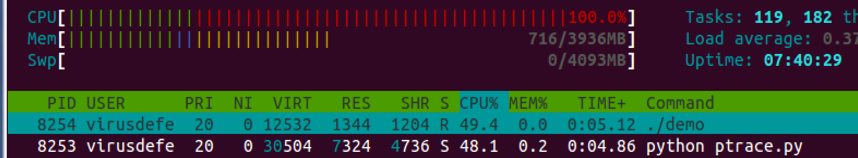
\includegraphics[width=0.9\textwidth]{ptrace-parent-process}
\caption{ptrace父进程也消耗大量CPU资源}
\end{figure}

测试环境:Ubuntu 14.04,虚拟化单核,主机MacBook Pro Intel(R) Core(TM) i5-4278U CPU @ 2.60GHz。

seccomp是一种侵入式策略,需要在代码执行之前加载,而不是ptrace那样在父进程中全部控制。开发过程中设计过几种加载seccomp的方法,但是都逐渐的发现存在绕过,最终方案是在\texttt{execve}之前加载,并且对\texttt{execve}这个本该是黑名单的系统调用进行了参数过滤,下面章节是详细的分析。

\subsubsection{动态库使用\texttt{LD\_PRELOAD}加载的绕过}

在编写代码的时候一般是从main函数开始的,但是实际进程执行的时候并不是,在main函数执行之前还有一些初始化函数,比如\texttt{start}和\texttt{\_\_libc\_start\_main}函数\cite{linux-process-start}。如果可以hook这些函数就可以在用户代码执行之前执行加载seccomp的代码了,很明显可以使用动态库来覆盖\texttt{\_\_libc\_start\_main},加载seccomp策略,然后模拟正常执行的去调用main函数,示例如下

\begin{verbatim}

typedef int (*main_t)(int, char **, char **);  
int __libc_start_main(main_t main, int argc, 
    char *__unbounded *__unbounded ubp_av,
    ElfW(auxv_t) *__unbounded auxvec,
    __typeof (main) init,
    void (*fini) (void),
    void (*rtld_fini) (void), void *__unbounded
    stack_end)
{
    int i;
    ssize_t len;
    void *libc;
    int (*libc_start_main)(main_t main,
        int,
        char *__unbounded *__unbounded,
        ElfW(auxv_t) *,
        __typeof (main),
        void (*fini) (void),
        void (*rtld_fini) (void),
        void *__unbounded stack_end);
    libc = dlopen("libc.so.6", RTLD_LOCAL  | RTLD_LAZY);
    if (!libc) {
        exit(1);
    }
  
    libc_start_main = dlsym(libc, "__libc_start_main");
    if (!libc_start_main) {
        exit(2);
}
// TODO: load seccomp rules
    return ((*libc_start_main)(main, argc, ubp_av, auxvec,
                 init, fini, rtld_fini, stack_end));
}

\end{verbatim}

上述代码由 https://github.com/quark-zju/lrun 修改而来,完整代码和编译选项可见GitHub。GitHub上另外一个项目 https://github.com/daveho/EasySandbox 也使用了类似的方法。并且EasySandbox的说明\cite{easy-sandbox-bypass}中也提到了这种实现可能的绕过:如果用户程序自定义了\\\texttt{\_\_libc\_start\_main}函数,动态库中的\texttt{\_\_libc\_start\_main}就不会执行,但是这个需要编译选项\texttt{-nostdlib}的支持,如果没有这个编译选项,就会出现编译错误。

将上述代码加载seccomp的部分删除,补充main函数,在Ubuntu 14.04上使用gcc 4.8.4进行编译并没有出现编译错误,并且执行的是确实是用户的而不是沙箱的\texttt{\_\_libc\_start\_main}函数,导致沙箱被绕过。所以这种方案只能放弃,如果没有这个问题,确实是一个很好的做法,不需要修改任何代码,只要加载一个动态库,后续的进程行为都被我们控制了。

\subsubsection{同名库函数覆盖导致的绕过}

为了避免\texttt{\_\_libc\_start\_main}函数被覆盖,可以将沙箱代码和用户代码一起编译,这样用户代码中如果也定义了\texttt{\_\_libc\_start\_main}就会导致编译错误,实际验证也是这样的。但是用户代码中也可以覆盖一些头文件中的函数为空函数,导致沙箱失效,比如\texttt{seccomp\_rule\_add}、\texttt{seccomp\_release}函数等。

\begin{verbatim}
#include <stdio.h>
#include <seccomp.h>

int seccomp_rule_add(scmp_filter_ctx ctx, uint32_t action, 
                     int syscall, unsigned int arg_cnt, ...) {
    printf("This is a fake seccomp_rule_add\n");
    return 0;
}
int seccomp_load(scmp_filter_ctx ctx) {
    return 0;
}
void seccomp_release(scmp_filter_ctx ctx) {}
int main()
{
    return 0;
}
\end{verbatim}

\texttt{gcc main.c sandbox.c -ldl -lseccomp -o user\_code \&\& ./user\_code}编译运行发现输出了This is a fake seccomp\_rule\_add。

\subsubsection{在\texttt{execve}之前加载seccomp}

在\texttt{execve}之前加载seccomp看起来是没有问题的,但是seccomp策略是白名单类型的,要这样做的话必须将\texttt{execve}也加入白名单,而这确确实实是一个危险函数,也可以直接用来执行系统命令,所以也是一个潜在的绕过,我们可以使用seccomp的参数过滤来过滤\texttt{execve}的参数,可执行文件路径只能是确定的。例如

\begin{verbatim}
#include <stdio.h>
#include <unistd.h>
#include <seccomp.h>
  
int main() {
  char file_name[30] = "/bin/ls";
  char dangerous_file_name[30] = "/bin/rm";
  char *argv[] = {"/", NULL};
  char *env[] = {NULL};
  scmp_filter_ctx ctx;
  ctx = seccomp_init(SCMP_ACT_ALLOW);
  seccomp_rule_add(ctx, SCMP_ACT_KILL, SCMP_SYS(execve), 1,
                        SCMP_A0(SCMP_CMP_NE, file_name));
  seccomp_load(ctx);
  execve(file_name, argv, env);
  return 0;
}
\end{verbatim}

如果把\texttt{file\_name}换成\texttt{dangerous\_file\_name},就会提示bad system call。这样就解决了\texttt{execve}可能带来的绕过。

\subsubsection{系统调用白名单}

确定了加载seccomp的方法之后,只需要确定哪些系统调用是安全的就可以了。在Linux系统下,使用\texttt{strace}命令可以获取进程运行所有的系统调用,在抽样分析了OJ上提交过的代码之后,得到了以下系统调用白名单。
\begin{table}[H]
\centering
\caption{系统调用白名单}
\begin{tabular}{ |c|c| } 
\hline
系统调用 & 说明 \\
\hline
open &打开一个文件 \\
\hline
read &读取文件 \\
\hline
write &写文件 \\
\hline
close &关闭文件 \\
\hline
fstat &检测文件状态 \\
\hline
mmap &\multirow{5}{4em}{内存分配相关} \\ 
munmap& \\ 
mprotect& \\ 
arch\_ptctl& \\
brk& \\
\hline
access &检查文件权限 \\
\hline
exit\_group &结束进程的所有线程 \\
\hline
\end{tabular}
\end{table}
和\texttt{execve}一样,\texttt{write}系统调用也需要过滤参数。当\texttt{write}的参数为1和2的时候,代表\texttt{stdout}和\texttt{strerr},其余的参数值代表某个文件的文件描述符,如果不限制\texttt{write}的参数,进程就可以写任意文件了。

使用了下面的代码实现

\begin{verbatim}
// only fd 0 1 2 are allowed
if (seccomp_rule_add(ctx, SCMP_ACT_ALLOW, SCMP_SYS(write), 1, 
                          SCMP_A0(SCMP_CMP_LE, 2))) {
    LOG_FATAL("load dup2 rule failed");
    ERROR(LOAD_SECCOMP_FAILED);
}
\end{verbatim}

\subsubsection{用户权限控制}

Linux上用户分为root用户和非root用户。root用户拥有最高权限,而nobody用户权限非常低,可以使用nobody用户来运行风险级别比较高的进程,比如各种Web服务器软件。沙箱也使用了这个用户来运行用户的代码,一旦沙箱机制被攻破,还可以通过Linux用户权限控制避免更大的危害。
Linux中提供了\texttt{setuid}函数,可以以uid用户身份运行,但是需要root权限来调用。

使用了下面的代码实现

\begin{verbatim}
if (setgid(NOBODY_GID)) {
    LOG_FATAL("setgid failed, errno: %d", errno);
    ERROR(SET_GID_FAILED);
}
if (setuid(NOBODY_UID)) {
    LOG_FATAL("setuid failed, errno: %d", errno);
    ERROR(SET_UID_FAILED);
}
\end{verbatim}

\subsubsection{编译器安全}

这是一个容易被忽视的方面,目前已知的主要有以下几种。

一是引用某些可以无限输出的文件,比如\texttt{\#include</dev/random>},编译器会一直读取,导致卡死。

二是让编译器产生大量的错误信息,比如下面一段代码,可以让g++编译器产生数G的错误日志。

\begin{verbatim}
int main()
{
    struct x struct z<x(x(x(x(x(x(x(x(x(x(x(x(x(x(x(y,x(y><y*,x(y*w>v<y*,w,x{}
    return 0;
}
\end{verbatim}

处理方法就是编译器运行的时候也要控制CPU时间和实际运行时间,同时使用编译器参数\texttt{-fmax-errors=N}来控制最大错误数量。

三是\texttt{C++}的模板元编程,部分代码是编译期执行的,可以构造出让编译器产生大量计算的代码。

和第二个问题一样,实际大量的去占用资源的并不是编译器进程,而是编译器的子进程,在单纯使用\texttt{setitimer}方法的时候并无法控制子进程,所以还需要\texttt{setrlimit}的辅助。

四是引用一些敏感文件可能导致信息泄露,比如\texttt{\#include</etc/shadow/>},会在编译错误的信息中泄露文件开头的内容。

\subsubsection{小结}
我们主要是从系统调用的层面来保证安全性的,而Linux还有很多其他的特性可以用来保证安全,比如\texttt{chroot}、\texttt{cgroups}、\texttt{user\_namespace}等。还可以将代码放入Docker或者虚拟机中运行,使用Docker或者虚拟机的隔离性进一步提高安全性。

在开发过程中还遇到了很多细节问题,如不同操作系统系统调用的不同,多线程竞态条件的问题等等。实现一个安全的判题沙箱是很困难的,需要对Linux API有深入的了解,有时还需要找源码或者反汇编查看一些底层的实现。
